\documentclass[17pt,a4paper,landscape]{extarticle}
\usepackage[margin=2.35cm,top=0.12cm,left=1.05cm]{geometry}
\usepackage{amsmath}
\usepackage{amssymb}
\usepackage{tasks}
\usepackage{tikz}
\usepackage{xcolor}
\usepackage[sfdefault,lf]{FiraSans}
\renewcommand{\familydefault}{\sfdefault}
\setlength{\parindent}{0pt}
\pagestyle{empty}
\settasks{label=\textbf{\arabic*.}, label-width=2.2em, item-indent=2.95em, column-sep=2.1cm, after-item-skip=4.7em}
\renewcommand{\arraystretch}{1.15}
\everymath{\displaystyle}

\begin{document}
\sffamily
\boldmath

\boldmath

\boldmath

\boldmath

\boldmath

{\LARGE \textbf{Finding point of intersection of two lines — Foundation}}\\[0.2em]
Read each graph and write the point where the two lines cross.

\begin{tasks}(3)
\task {Write the point of intersection: \mbox{$(\underline{\hspace{1.6cm}}, \underline{\hspace{1.6cm}})$}. \\[0.4em] 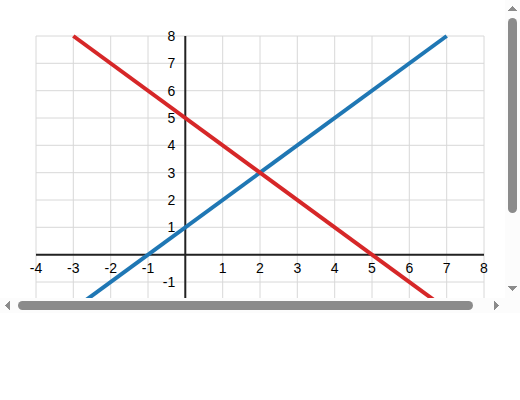
\includegraphics[width=0.88\linewidth]{web-diagrams/foundation-01.png}}
\task {Write the point of intersection: \mbox{$(\underline{\hspace{1.6cm}}, \underline{\hspace{1.6cm}})$}. \\[0.4em] 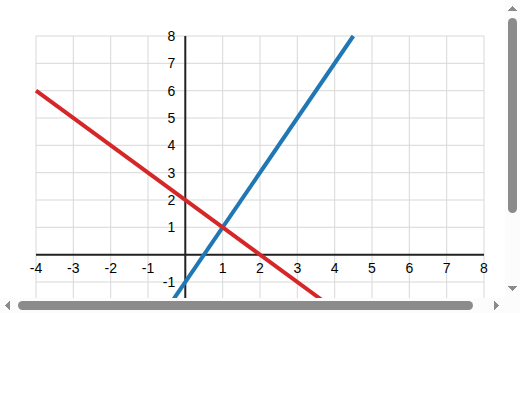
\includegraphics[width=0.88\linewidth]{web-diagrams/foundation-02.png}}
\task {Write the point of intersection: \mbox{$(\underline{\hspace{1.6cm}}, \underline{\hspace{1.6cm}})$}. \\[0.4em] 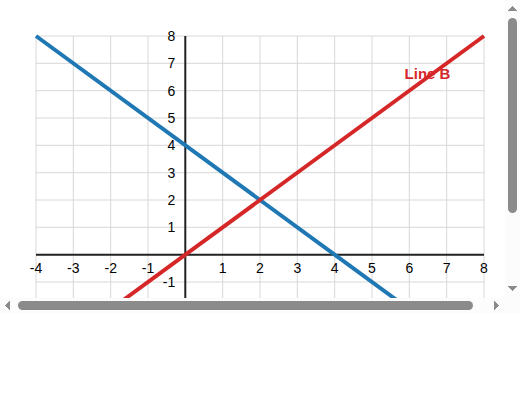
\includegraphics[width=0.88\linewidth]{web-diagrams/foundation-03.png}}
\task {Write the point of intersection: \mbox{$(\underline{\hspace{1.6cm}}, \underline{\hspace{1.6cm}})$}. \\[0.4em] 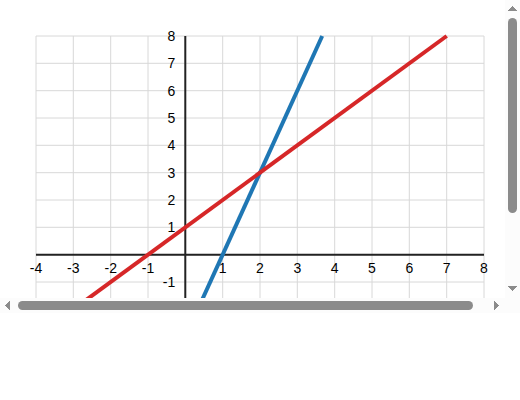
\includegraphics[width=0.88\linewidth]{web-diagrams/foundation-04.png}}
\task {Write the point of intersection: \mbox{$(\underline{\hspace{1.6cm}}, \underline{\hspace{1.6cm}})$}. \\[0.4em] 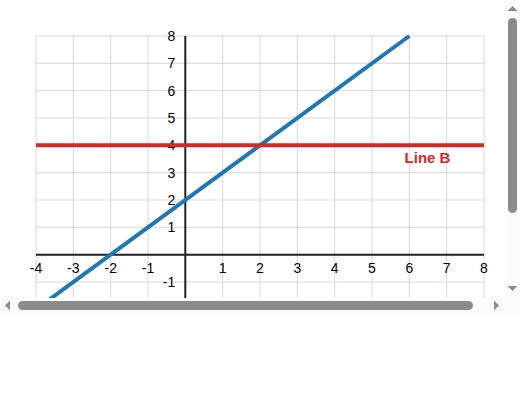
\includegraphics[width=0.88\linewidth]{web-diagrams/foundation-05.png}}
\task {Write the point of intersection: \mbox{$(\underline{\hspace{1.6cm}}, \underline{\hspace{1.6cm}})$}. \\[0.4em] 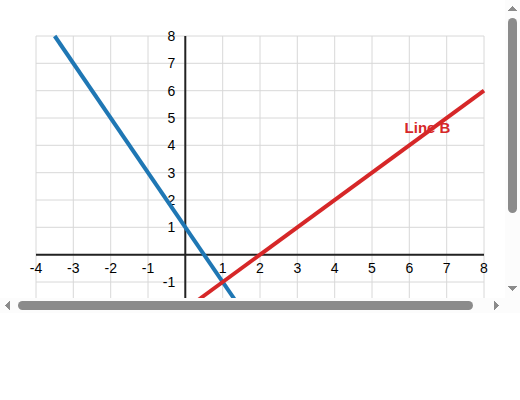
\includegraphics[width=0.88\linewidth]{web-diagrams/foundation-06.png}}
\task {Write the point of intersection: \mbox{$(\underline{\hspace{1.6cm}}, \underline{\hspace{1.6cm}})$}. \\[0.4em] 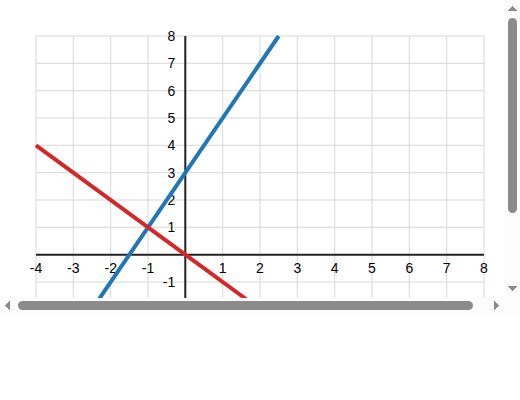
\includegraphics[width=0.88\linewidth]{web-diagrams/foundation-07.png}}
\task {Write the point of intersection: \mbox{$(\underline{\hspace{1.6cm}}, \underline{\hspace{1.6cm}})$}. \\[0.4em] 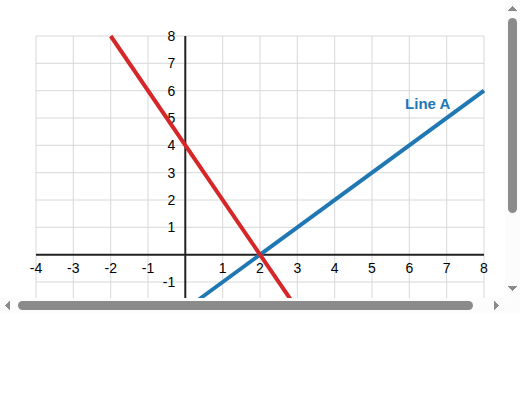
\includegraphics[width=0.88\linewidth]{web-diagrams/foundation-08.png}}
\task {Write the point of intersection: \mbox{$(\underline{\hspace{1.6cm}}, \underline{\hspace{1.6cm}})$}. \\[0.4em] 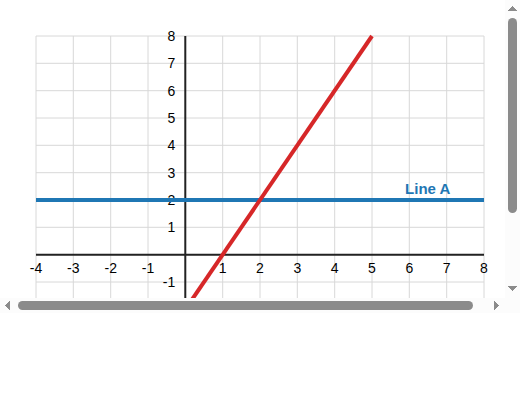
\includegraphics[width=0.88\linewidth]{web-diagrams/foundation-09.png}}
\task {Write the point of intersection: \mbox{$(\underline{\hspace{1.6cm}}, \underline{\hspace{1.6cm}})$}. \\[0.4em] 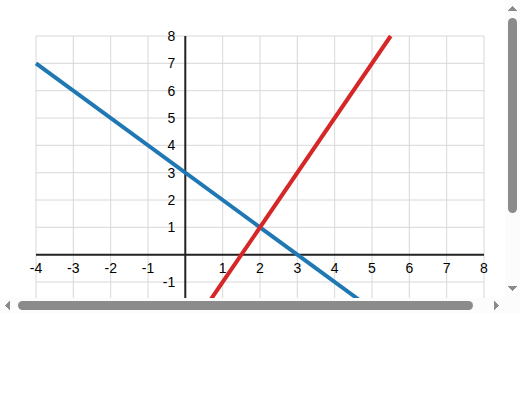
\includegraphics[width=0.88\linewidth]{web-diagrams/foundation-10.png}}
\task {Write the point of intersection: \mbox{$(\underline{\hspace{1.6cm}}, \underline{\hspace{1.6cm}})$}. \\[0.4em] 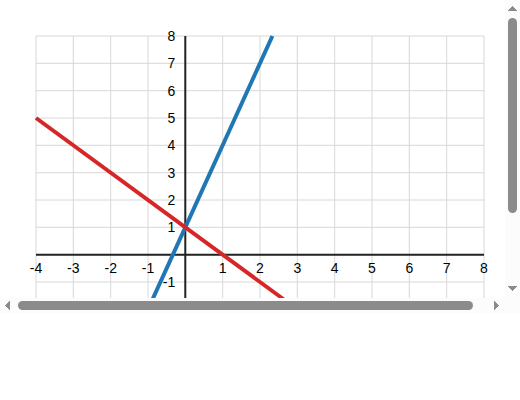
\includegraphics[width=0.88\linewidth]{web-diagrams/foundation-11.png}}
\task {Write the point of intersection: \mbox{$(\underline{\hspace{1.6cm}}, \underline{\hspace{1.6cm}})$}. \\[0.4em] 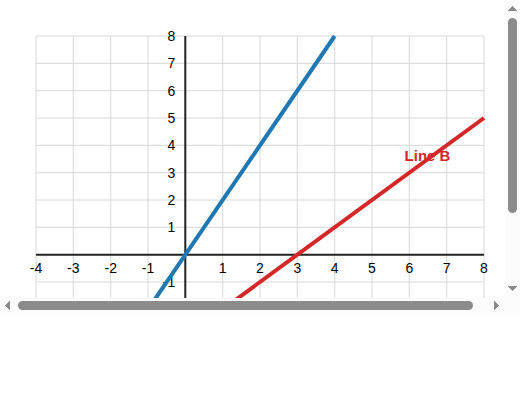
\includegraphics[width=0.88\linewidth]{web-diagrams/foundation-12.png}}
\end{tasks}

\end{document}
